\documentclass[12pt]{article}
\usepackage[utf8]{inputenc}
\usepackage[T1]{fontenc}
\usepackage{pdflscape} 
\usepackage{lmodern}
\usepackage[a4paper,bindingoffset=0.2in,%
            left=0.5in,right=0.5in,top=0.5in,bottom=1in,%
            footskip=.25in]{geometry}
\usepackage[colorlinks=true, linkcolor=Black, urlcolor=Blue]{hyperref}
\usepackage{graphicx}
\usepackage{subcaption}
\usepackage{listings}
\usepackage{color}
\usepackage[table]{xcolor}
\definecolor{lightgray}{gray}{0.9}

\definecolor{codegreen}{rgb}{0,0.6,0}
\definecolor{codegray}{rgb}{0.5,0.5,0.5}
\definecolor{codepurple}{rgb}{0.58,0,0.82}
\definecolor{backcolour}{rgb}{0.95,0.95,0.92}

\lstdefinestyle{mystyle}{
	backgroundcolor=\color{backcolour},   
	commentstyle=\color{codegreen},
	keywordstyle=\color{magenta},
	numberstyle=\tiny\color{codegray},
	stringstyle=\color{codepurple},
	basicstyle=\ttfamily\footnotesize,
	breakatwhitespace=false,         
	breaklines=true,                 
	captionpos=b,                    
	keepspaces=true,                 
	numbers=left,                    
	numbersep=5pt,                  
	showspaces=false,                
	showstringspaces=false,
	showtabs=false,                  
	tabsize=2
}


\begin{document}
\title{Projekt - Drzewa Decyzyjne I\\
\large Sebastian Michoń 136770, Marcin Zatorski 136834\\
\large grupe L5}
\date{\vspace{-10ex}}
\maketitle

\section{Metoda ogólna - dane dyskretne}
\begin{enumerate}
	\item Wpierw dataset jest wczytany do formatu dataframe biblioteki pandas. Usuwane są nazwiska pasażerów i ich nry id.
	
	\item Wiek pasażera jest transformowany zgodnie z wytycznymi (to dotyczy tylko obliczeń dla 1. części projektu).
	
	\item Drzewo jest tworzone jako tablica podzbiorów dataframe'a: na początku, w korzeniu drzewa (w 0. elemencie listy) dany jest cały dataframe; jeśli możliwy jest split w danym wierzchołku (i gain ratio wynikający z tego splita jest większy od 0), to dataframe w wierzchołku jest dzielony według kolumny, split na której daje najwyższy gain ratio. Każdy powstający podzbiór dataframe'a jest dodawany na koniec tablicy wierzchołków. Razem z nimi dla każdego wierzchołka uzyskuję informacje o nrze ojca i splicie, w wyniku którego powstał (który jest wygodny do późniejszego rysowania drzewa).
	
	\item Entropia, entropia warunkowa, gain ratio, information gain i intristic information są liczone jawnie ze wzoru - w ogólności złożoność obliczeniowa kalkulowania kolejnego splita to \(O(n\sum_{i=0}^{m}{x_i})\), gdzie \(n\) to liczba wierszy dataseta w danym wierzchołku, \(m\) to liczba atrybutów, a \(x_i\) to liczba różnych wartości w \(i\)-tym atrybucie dla dataframe'a w tym wierzchołku.
	
	\item W momencie, w którym nie da się uzyskać lepszego od 0 gain ratio w danym wierzchołku (może zajść, gdy żadna pojedyncza kolumna nie pozwala lepiej sklasyfikować zbioru danych niż sam wierzchołek), nie jest dokonywany żaden split (co nie oznacza, że nie byłoby zasadnym go dokonać - natomiast algorytm podziału jest zachłanny, więc działa w taki a nie inny sposób). Jeśli nie da się dokonać żadnego kolejnego splita konstrukcja drzewa się kończy. Przykład dataseta, w którym 2 splity prowadziłyby do wzrostu współczynnika informacji, choć żaden nie zostanie wykonany: (Y to atrybut, którego wartość chcemy poznać w zależności od c1, c2)\\
		\begin{tabular}{lll}
			c1 &  c2 &  Y \\
			A & B & 1 \\
			B & A & 1 \\
			A & A & 0 \\ 
			B & B & 0 \\ 
		\end{tabular}
	
	\item W ostatniej fazie rysowane jest drzewo - w osobnym pliku otwierającym się na poziomie jupytera, jako że wygodniej jest przeglądać duży obrazek właśnie w takiej formie niż jako standardowy obrazek wewnątrz jupytera; wierzchołek opisany jest w formacie "1:x / 0:y", który oznacza, że w wierzchołku jest x obserwacji mających w polu "Survived" wartość 1 i y obserwacji mających w polu "Survived" wartość 0. Na krawędzi pokazywany jest split który do powstania tego wierzchołka doprowadził.
\end{enumerate}

\section{Metoda dla danych ciągłych}
\begin{enumerate}
	\item Dla danych ciągłych split na atrybucie C dzieli zbiór obserwacji na 2 części: Obserwacje z wartością \(x\) atrybutu C: \(x \le f\) i obserwacje z wartością \(x\) atrybutu C: \(x > f\) dla \(f\) nazywanego dalej miejscem splita.
	\item Miejsce splita jest wybierane jako takie miejsce, podział w którym maksymalizuje gain ratio. Proba znalezienia gain ratio opisanym powyżej (dla danych dyskretnych) algorytmem działałaby w złożoności \(O(n^2)\) dla \(n\) będącego liczbą wierszy dataseta, co jest niestaysfakcjonujące.
	\item Można także posortować dataset po atrybucie C, przesuwać potencjalne \(f\) do przodu, modyfikując dynamicznie listy wartości do obliczania warunkowej entropii i intristic info w czasie stałym i kalkulować je także w czasie stałym - złożoność zatem wyniesie \(O(nlog(n))\)
\end{enumerate}

\section{Działanie algorytmu - Logi (wersja na 5.0)}
W kolejnych wierszach: wszystkie gain ratio dla atrybutów, w \# wybrany atrybut do podziału, w przypadku atrybutu ciągłego punkt splita dający daną wartość gain ratio
\begin{verbatim}
	New vertex is processed: this vertex contains
	- 40 survived observations
	- 60 deceased observations
	The splits that led to the advent of this vertex were:
	[]
	column: Pclass, gain ratio: 0.05960489889898, attribute discrete
	column: Sex, gain ratio: 0.40323636523376316, attribute discrete
	column: Age, gain ratio: 0.16497395662937295, split value: 1
	column: SibSp, gain ratio: 0.02511018959580578, attribute discrete
	column: Parch, gain ratio: 0.01464001497707953, attribute discrete
	############### Chosen attribute: Sex, value of gain: 0.40323636523376316
	
	New vertex is processed: this vertex contains
	- 7 survived observations
	- 53 deceased observations
	The splits that led to the advent of this vertex were:
	['Sex = male']
	column: Pclass, gain ratio: 0.07729306659385578, attribute discrete
	column: Sex, gain ratio: 0.0, attribute discrete
	column: Age, gain ratio: 0.4355418320733391, split value: 1
	column: SibSp, gain ratio: 0.020306536706473522, attribute discrete
	column: Parch, gain ratio: 0.03512786197394762, attribute discrete
	############### Chosen attribute: Age, value of gain: 0.4355418320733391
	
	New vertex is processed: this vertex contains
	- 33 survived observations
	- 7 deceased observations
	The splits that led to the advent of this vertex were:
	['Sex = female']
	column: Pclass, gain ratio: 0.12003370114124165, attribute discrete
	column: Sex, gain ratio: 0.0, attribute discrete
	column: Age, gain ratio: 0.08066119202255055, split value: 40
	column: SibSp, gain ratio: 0.16649361093302303, attribute discrete
	column: Parch, gain ratio: 0.013322955978332338, attribute discrete
	############### Chosen attribute: SibSp, value of gain: 0.16649361093302303
	
	New vertex is processed: this vertex contains
	- 1 survived observations
	- 0 deceased observations
	The splits that led to the advent of this vertex were:
	['Sex = male', 'Age <= 1']
	column: Pclass, gain ratio: 0.0, attribute discrete
	column: Sex, gain ratio: 0.0, attribute discrete
	column: Age, gain ratio: 0, split value: 0
	column: SibSp, gain ratio: 0.0, attribute discrete
	column: Parch, gain ratio: 0.0, attribute discrete
	############### No chosen attribute, end of processing for this subset of dataframe
	
	New vertex is processed: this vertex contains
	- 6 survived observations
	- 53 deceased observations
	The splits that led to the advent of this vertex were:
	['Sex = male', 'Age > 1']
	column: Pclass, gain ratio: 0.07134448543370803, attribute discrete
	column: Sex, gain ratio: 0.0, attribute discrete
	column: Age, gain ratio: 0.05346216522701795, split value: 40
	column: SibSp, gain ratio: 0.016521875902366145, attribute discrete
	column: Parch, gain ratio: 0.0438446848069315, attribute discrete
	############### Chosen attribute: Pclass, value of gain: 0.07134448543370803
	
	New vertex is processed: this vertex contains
	- 11 survived observations
	- 4 deceased observations
	The splits that led to the advent of this vertex were:
	['Sex = female', 'SibSp = 1']
	column: Pclass, gain ratio: 0.2997723162709534, attribute discrete
	column: Sex, gain ratio: 0.0, attribute discrete
	column: Age, gain ratio: 0.17110871057416346, split value: 14
	column: SibSp, gain ratio: 0.0, attribute discrete
	column: Parch, gain ratio: 0.11576241483250045, attribute discrete
	############### Chosen attribute: Pclass, value of gain: 0.2997723162709534
	
	New vertex is processed: this vertex contains
	- 19 survived observations
	- 0 deceased observations
	The splits that led to the advent of this vertex were:
	['Sex = female', 'SibSp = 0']
	column: Pclass, gain ratio: 0.0, attribute discrete
	column: Sex, gain ratio: 0.0, attribute discrete
	column: Age, gain ratio: 0, split value: 0
	column: SibSp, gain ratio: 0.0, attribute discrete
	column: Parch, gain ratio: 0.0, attribute discrete
	############### No chosen attribute, end of processing for this subset of dataframe
	
	New vertex is processed: this vertex contains
	- 2 survived observations
	- 1 deceased observations
	The splits that led to the advent of this vertex were:
	['Sex = female', 'SibSp = 3']
	column: Pclass, gain ratio: 0.274017542121281, attribute discrete
	column: Sex, gain ratio: 0.0, attribute discrete
	column: Age, gain ratio: 1.0, split value: 8
	column: SibSp, gain ratio: 0.0, attribute discrete
	column: Parch, gain ratio: 0.579380164285695, attribute discrete
	############### Chosen attribute: Age, value of gain: 1.0
	
	New vertex is processed: this vertex contains
	- 0 survived observations
	- 1 deceased observations
	The splits that led to the advent of this vertex were:
	['Sex = female', 'SibSp = 2']
	column: Pclass, gain ratio: 0.0, attribute discrete
	column: Sex, gain ratio: 0.0, attribute discrete
	column: Age, gain ratio: 0, split value: 0
	column: SibSp, gain ratio: 0.0, attribute discrete
	column: Parch, gain ratio: 0.0, attribute discrete
	############### No chosen attribute, end of processing for this subset of dataframe
	
	New vertex is processed: this vertex contains
	- 1 survived observations
	- 0 deceased observations
	The splits that led to the advent of this vertex were:
	['Sex = female', 'SibSp = 4']
	column: Pclass, gain ratio: 0.0, attribute discrete
	column: Sex, gain ratio: 0.0, attribute discrete
	column: Age, gain ratio: 0, split value: 0
	column: SibSp, gain ratio: 0.0, attribute discrete
	column: Parch, gain ratio: 0.0, attribute discrete
	############### No chosen attribute, end of processing for this subset of dataframe
	
	New vertex is processed: this vertex contains
	- 0 survived observations
	- 1 deceased observations
	The splits that led to the advent of this vertex were:
	['Sex = female', 'SibSp = 5']
	column: Pclass, gain ratio: 0.0, attribute discrete
	column: Sex, gain ratio: 0.0, attribute discrete
	column: Age, gain ratio: 0, split value: 0
	column: SibSp, gain ratio: 0.0, attribute discrete
	column: Parch, gain ratio: 0.0, attribute discrete
	############### No chosen attribute, end of processing for this subset of dataframe
	
	New vertex is processed: this vertex contains
	- 1 survived observations
	- 37 deceased observations
	The splits that led to the advent of this vertex were:
	['Sex = male', 'Age > 1', 'Pclass = 3']
	column: Pclass, gain ratio: 0.0, attribute discrete
	column: Sex, gain ratio: 0.0, attribute discrete
	column: Age, gain ratio: 0.05569120277229924, split value: 32
	column: SibSp, gain ratio: 0.03969457544077502, attribute discrete
	column: Parch, gain ratio: 0.07483597867418908, attribute discrete
	############### Chosen attribute: Parch, value of gain: 0.07483597867418908
	
	New vertex is processed: this vertex contains
	- 4 survived observations
	- 9 deceased observations
	The splits that led to the advent of this vertex were:
	['Sex = male', 'Age > 1', 'Pclass = 1']
	column: Pclass, gain ratio: 0.0, attribute discrete
	column: Sex, gain ratio: 0.0, attribute discrete
	column: Age, gain ratio: 0.4686651882055394, split value: 40
	column: SibSp, gain ratio: 0.222057265152258, attribute discrete
	column: Parch, gain ratio: 0.059246976190095675, attribute discrete
	############### Chosen attribute: Age, value of gain: 0.4686651882055394
	
	New vertex is processed: this vertex contains
	- 1 survived observations
	- 7 deceased observations
	The splits that led to the advent of this vertex were:
	['Sex = male', 'Age > 1', 'Pclass = 2']
	column: Pclass, gain ratio: 0.0, attribute discrete
	column: Sex, gain ratio: 0.0, attribute discrete
	column: Age, gain ratio: 1.0, split value: 12
	column: SibSp, gain ratio: 0.04755786045881497, attribute discrete
	column: Parch, gain ratio: 0.0, attribute discrete
	############### Chosen attribute: Age, value of gain: 1.0
	
	New vertex is processed: this vertex contains
	- 4 survived observations
	- 0 deceased observations
	The splits that led to the advent of this vertex were:
	['Sex = female', 'SibSp = 1', 'Pclass = 1']
	column: Pclass, gain ratio: 0.0, attribute discrete
	column: Sex, gain ratio: 0.0, attribute discrete
	column: Age, gain ratio: 0, split value: 0
	column: SibSp, gain ratio: 0.0, attribute discrete
	column: Parch, gain ratio: 0.0, attribute discrete
	############### No chosen attribute, end of processing for this subset of dataframe
	
	New vertex is processed: this vertex contains
	- 5 survived observations
	- 0 deceased observations
	The splits that led to the advent of this vertex were:
	['Sex = female', 'SibSp = 1', 'Pclass = 2']
	column: Pclass, gain ratio: 0.0, attribute discrete
	column: Sex, gain ratio: 0.0, attribute discrete
	column: Age, gain ratio: 0, split value: 0
	column: SibSp, gain ratio: 0.0, attribute discrete
	column: Parch, gain ratio: 0.0, attribute discrete
	############### No chosen attribute, end of processing for this subset of dataframe
	
	New vertex is processed: this vertex contains
	- 2 survived observations
	- 4 deceased observations
	The splits that led to the advent of this vertex were:
	['Sex = female', 'SibSp = 1', 'Pclass = 3']
	column: Pclass, gain ratio: 0.0, attribute discrete
	column: Sex, gain ratio: 0.0, attribute discrete
	column: Age, gain ratio: 0.4871971762327021, split value: 4
	column: SibSp, gain ratio: 0.0, attribute discrete
	column: Parch, gain ratio: 0.7336804366512111, attribute discrete
	############### Chosen attribute: Parch, value of gain: 0.7336804366512111
	
	New vertex is processed: this vertex contains
	- 0 survived observations
	- 1 deceased observations
	The splits that led to the advent of this vertex were:
	['Sex = female', 'SibSp = 3', 'Age <= 8']
	column: Pclass, gain ratio: 0.0, attribute discrete
	column: Sex, gain ratio: 0.0, attribute discrete
	column: Age, gain ratio: 0, split value: 0
	column: SibSp, gain ratio: 0.0, attribute discrete
	column: Parch, gain ratio: 0.0, attribute discrete
	############### No chosen attribute, end of processing for this subset of dataframe
	
	New vertex is processed: this vertex contains
	- 2 survived observations
	- 0 deceased observations
	The splits that led to the advent of this vertex were:
	['Sex = female', 'SibSp = 3', 'Age > 8']
	column: Pclass, gain ratio: 0.0, attribute discrete
	column: Sex, gain ratio: 0.0, attribute discrete
	column: Age, gain ratio: 0, split value: 0
	column: SibSp, gain ratio: 0.0, attribute discrete
	column: Parch, gain ratio: 0.0, attribute discrete
	############### No chosen attribute, end of processing for this subset of dataframe
	
	New vertex is processed: this vertex contains
	- 0 survived observations
	- 29 deceased observations
	The splits that led to the advent of this vertex were:
	['Sex = male', 'Age > 1', 'Pclass = 3', 'Parch = 0']
	column: Pclass, gain ratio: 0.0, attribute discrete
	column: Sex, gain ratio: 0.0, attribute discrete
	column: Age, gain ratio: 0, split value: 0
	column: SibSp, gain ratio: 0.0, attribute discrete
	column: Parch, gain ratio: 0.0, attribute discrete
	############### No chosen attribute, end of processing for this subset of dataframe
	
	New vertex is processed: this vertex contains
	- 1 survived observations
	- 3 deceased observations
	The splits that led to the advent of this vertex were:
	['Sex = male', 'Age > 1', 'Pclass = 3', 'Parch = 1']
	column: Pclass, gain ratio: 0.0, attribute discrete
	column: Sex, gain ratio: 0.0, attribute discrete
	column: Age, gain ratio: 1.0, split value: 7
	column: SibSp, gain ratio: 0.5408520829727552, attribute discrete
	column: Parch, gain ratio: 0.0, attribute discrete
	############### Chosen attribute: Age, value of gain: 1.0
	
	New vertex is processed: this vertex contains
	- 0 survived observations
	- 1 deceased observations
	The splits that led to the advent of this vertex were:
	['Sex = male', 'Age > 1', 'Pclass = 3', 'Parch = 5']
	column: Pclass, gain ratio: 0.0, attribute discrete
	column: Sex, gain ratio: 0.0, attribute discrete
	column: Age, gain ratio: 0, split value: 0
	column: SibSp, gain ratio: 0.0, attribute discrete
	column: Parch, gain ratio: 0.0, attribute discrete
	############### No chosen attribute, end of processing for this subset of dataframe
	
	New vertex is processed: this vertex contains
	- 0 survived observations
	- 3 deceased observations
	The splits that led to the advent of this vertex were:
	['Sex = male', 'Age > 1', 'Pclass = 3', 'Parch = 2']
	column: Pclass, gain ratio: 0.0, attribute discrete
	column: Sex, gain ratio: 0.0, attribute discrete
	column: Age, gain ratio: 0, split value: 0
	column: SibSp, gain ratio: 0.0, attribute discrete
	column: Parch, gain ratio: 0.0, attribute discrete
	############### No chosen attribute, end of processing for this subset of dataframe
	
	New vertex is processed: this vertex contains
	- 0 survived observations
	- 1 deceased observations
	The splits that led to the advent of this vertex were:
	['Sex = male', 'Age > 1', 'Pclass = 3', 'Parch = 3']
	column: Pclass, gain ratio: 0.0, attribute discrete
	column: Sex, gain ratio: 0.0, attribute discrete
	column: Age, gain ratio: 0, split value: 0
	column: SibSp, gain ratio: 0.0, attribute discrete
	column: Parch, gain ratio: 0.0, attribute discrete
	############### No chosen attribute, end of processing for this subset of dataframe
	
	New vertex is processed: this vertex contains
	- 4 survived observations
	- 2 deceased observations
	The splits that led to the advent of this vertex were:
	['Sex = male', 'Age > 1', 'Pclass = 1', 'Age <= 40']
	column: Pclass, gain ratio: 0.0, attribute discrete
	column: Sex, gain ratio: 0.0, attribute discrete
	column: Age, gain ratio: 0.16794857383343836, split value: 13
	column: SibSp, gain ratio: 0.7336804366512111, attribute discrete
	column: Parch, gain ratio: 0.3015619649304495, attribute discrete
	############### Chosen attribute: SibSp, value of gain: 0.7336804366512111
	
	New vertex is processed: this vertex contains
	- 0 survived observations
	- 7 deceased observations
	The splits that led to the advent of this vertex were:
	['Sex = male', 'Age > 1', 'Pclass = 1', 'Age > 40']
	column: Pclass, gain ratio: 0.0, attribute discrete
	column: Sex, gain ratio: 0.0, attribute discrete
	column: Age, gain ratio: 0, split value: 0
	column: SibSp, gain ratio: 0.0, attribute discrete
	column: Parch, gain ratio: 0.0, attribute discrete
	############### No chosen attribute, end of processing for this subset of dataframe
	
	New vertex is processed: this vertex contains
	- 1 survived observations
	- 0 deceased observations
	The splits that led to the advent of this vertex were:
	['Sex = male', 'Age > 1', 'Pclass = 2', 'Age <= 12']
	column: Pclass, gain ratio: 0.0, attribute discrete
	column: Sex, gain ratio: 0.0, attribute discrete
	column: Age, gain ratio: 0, split value: 0
	column: SibSp, gain ratio: 0.0, attribute discrete
	column: Parch, gain ratio: 0.0, attribute discrete
	############### No chosen attribute, end of processing for this subset of dataframe
	
	New vertex is processed: this vertex contains
	- 0 survived observations
	- 7 deceased observations
	The splits that led to the advent of this vertex were:
	['Sex = male', 'Age > 1', 'Pclass = 2', 'Age > 12']
	column: Pclass, gain ratio: 0.0, attribute discrete
	column: Sex, gain ratio: 0.0, attribute discrete
	column: Age, gain ratio: 0, split value: 0
	column: SibSp, gain ratio: 0.0, attribute discrete
	column: Parch, gain ratio: 0.0, attribute discrete
	############### No chosen attribute, end of processing for this subset of dataframe
	
	New vertex is processed: this vertex contains
	- 1 survived observations
	- 0 deceased observations
	The splits that led to the advent of this vertex were:
	['Sex = female', 'SibSp = 1', 'Pclass = 3', 'Parch = 1']
	column: Pclass, gain ratio: 0.0, attribute discrete
	column: Sex, gain ratio: 0.0, attribute discrete
	column: Age, gain ratio: 0, split value: 0
	column: SibSp, gain ratio: 0.0, attribute discrete
	column: Parch, gain ratio: 0.0, attribute discrete
	############### No chosen attribute, end of processing for this subset of dataframe
	
	New vertex is processed: this vertex contains
	- 0 survived observations
	- 4 deceased observations
	The splits that led to the advent of this vertex were:
	['Sex = female', 'SibSp = 1', 'Pclass = 3', 'Parch = 0']
	column: Pclass, gain ratio: 0.0, attribute discrete
	column: Sex, gain ratio: 0.0, attribute discrete
	column: Age, gain ratio: 0, split value: 0
	column: SibSp, gain ratio: 0.0, attribute discrete
	column: Parch, gain ratio: 0.0, attribute discrete
	############### No chosen attribute, end of processing for this subset of dataframe
	
	New vertex is processed: this vertex contains
	- 1 survived observations
	- 0 deceased observations
	The splits that led to the advent of this vertex were:
	['Sex = female', 'SibSp = 1', 'Pclass = 3', 'Parch = 5']
	column: Pclass, gain ratio: 0.0, attribute discrete
	column: Sex, gain ratio: 0.0, attribute discrete
	column: Age, gain ratio: 0, split value: 0
	column: SibSp, gain ratio: 0.0, attribute discrete
	column: Parch, gain ratio: 0.0, attribute discrete
	############### No chosen attribute, end of processing for this subset of dataframe
	
	New vertex is processed: this vertex contains
	- 0 survived observations
	- 3 deceased observations
	The splits that led to the advent of this vertex were:
	['Sex = male', 'Age > 1', 'Pclass = 3', 'Parch = 1', 'Age <= 7']
	
	column: Pclass, gain ratio: 0.0, attribute discrete
	column: Sex, gain ratio: 0.0, attribute discrete
	column: Age, gain ratio: 0, split value: 0
	column: SibSp, gain ratio: 0.0, attribute discrete
	column: Parch, gain ratio: 0.0, attribute discrete
	############### No chosen attribute, end of processing for this subset of dataframe
	
	New vertex is processed: this vertex contains
	- 1 survived observations
	- 0 deceased observations
	The splits that led to the advent of this vertex were:
	['Sex = male', 'Age > 1', 'Pclass = 3', 'Parch = 1', 'Age > 7']
	column: Pclass, gain ratio: 0.0, attribute discrete
	column: Sex, gain ratio: 0.0, attribute discrete
	column: Age, gain ratio: 0, split value: 0
	column: SibSp, gain ratio: 0.0, attribute discrete
	column: Parch, gain ratio: 0.0, attribute discrete
	############### No chosen attribute, end of processing for this subset of dataframe
	
	New vertex is processed: this vertex contains
	- 4 survived observations
	- 0 deceased observations
	The splits that led to the advent of this vertex were:
	['Sex = male', 'Age > 1', 'Pclass = 1', 'Age <= 40', 'SibSp = 0']
	column: Pclass, gain ratio: 0.0, attribute discrete
	column: Sex, gain ratio: 0.0, attribute discrete
	column: Age, gain ratio: 0, split value: 0
	column: SibSp, gain ratio: 0.0, attribute discrete
	column: Parch, gain ratio: 0.0, attribute discrete
	############### No chosen attribute, end of processing for this subset of dataframe
	
	New vertex is processed: this vertex contains
	- 0 survived observations
	- 1 deceased observations
	The splits that led to the advent of this vertex were:
	['Sex = male', 'Age > 1', 'Pclass = 1', 'Age <= 40', 'SibSp = 3']
	column: Pclass, gain ratio: 0.0, attribute discrete
	column: Sex, gain ratio: 0.0, attribute discrete
	column: Age, gain ratio: 0, split value: 0
	column: SibSp, gain ratio: 0.0, attribute discrete
	column: Parch, gain ratio: 0.0, attribute discrete
	############### No chosen attribute, end of processing for this subset of dataframe
	
	New vertex is processed: this vertex contains
	- 0 survived observations
	- 1 deceased observations
	The splits that led to the advent of this vertex were:
	['Sex = male', 'Age > 1', 'Pclass = 1', 'Age <= 40', 'SibSp = 1']
	column: Pclass, gain ratio: 0.0, attribute discrete
	column: Sex, gain ratio: 0.0, attribute discrete
	column: Age, gain ratio: 0, split value: 0
	column: SibSp, gain ratio: 0.0, attribute discrete
	column: Parch, gain ratio: 0.0, attribute discrete
	############### No chosen attribute, end of processing for this subset of dataframe
	
	
\end{verbatim}
\section{Działanie algorytmu - Generowane drzewa}

\begin{figure}[h!]
	\subsection{Dyskretny Age}
	\centering
	\begin{subfigure}[b]{1\linewidth}
		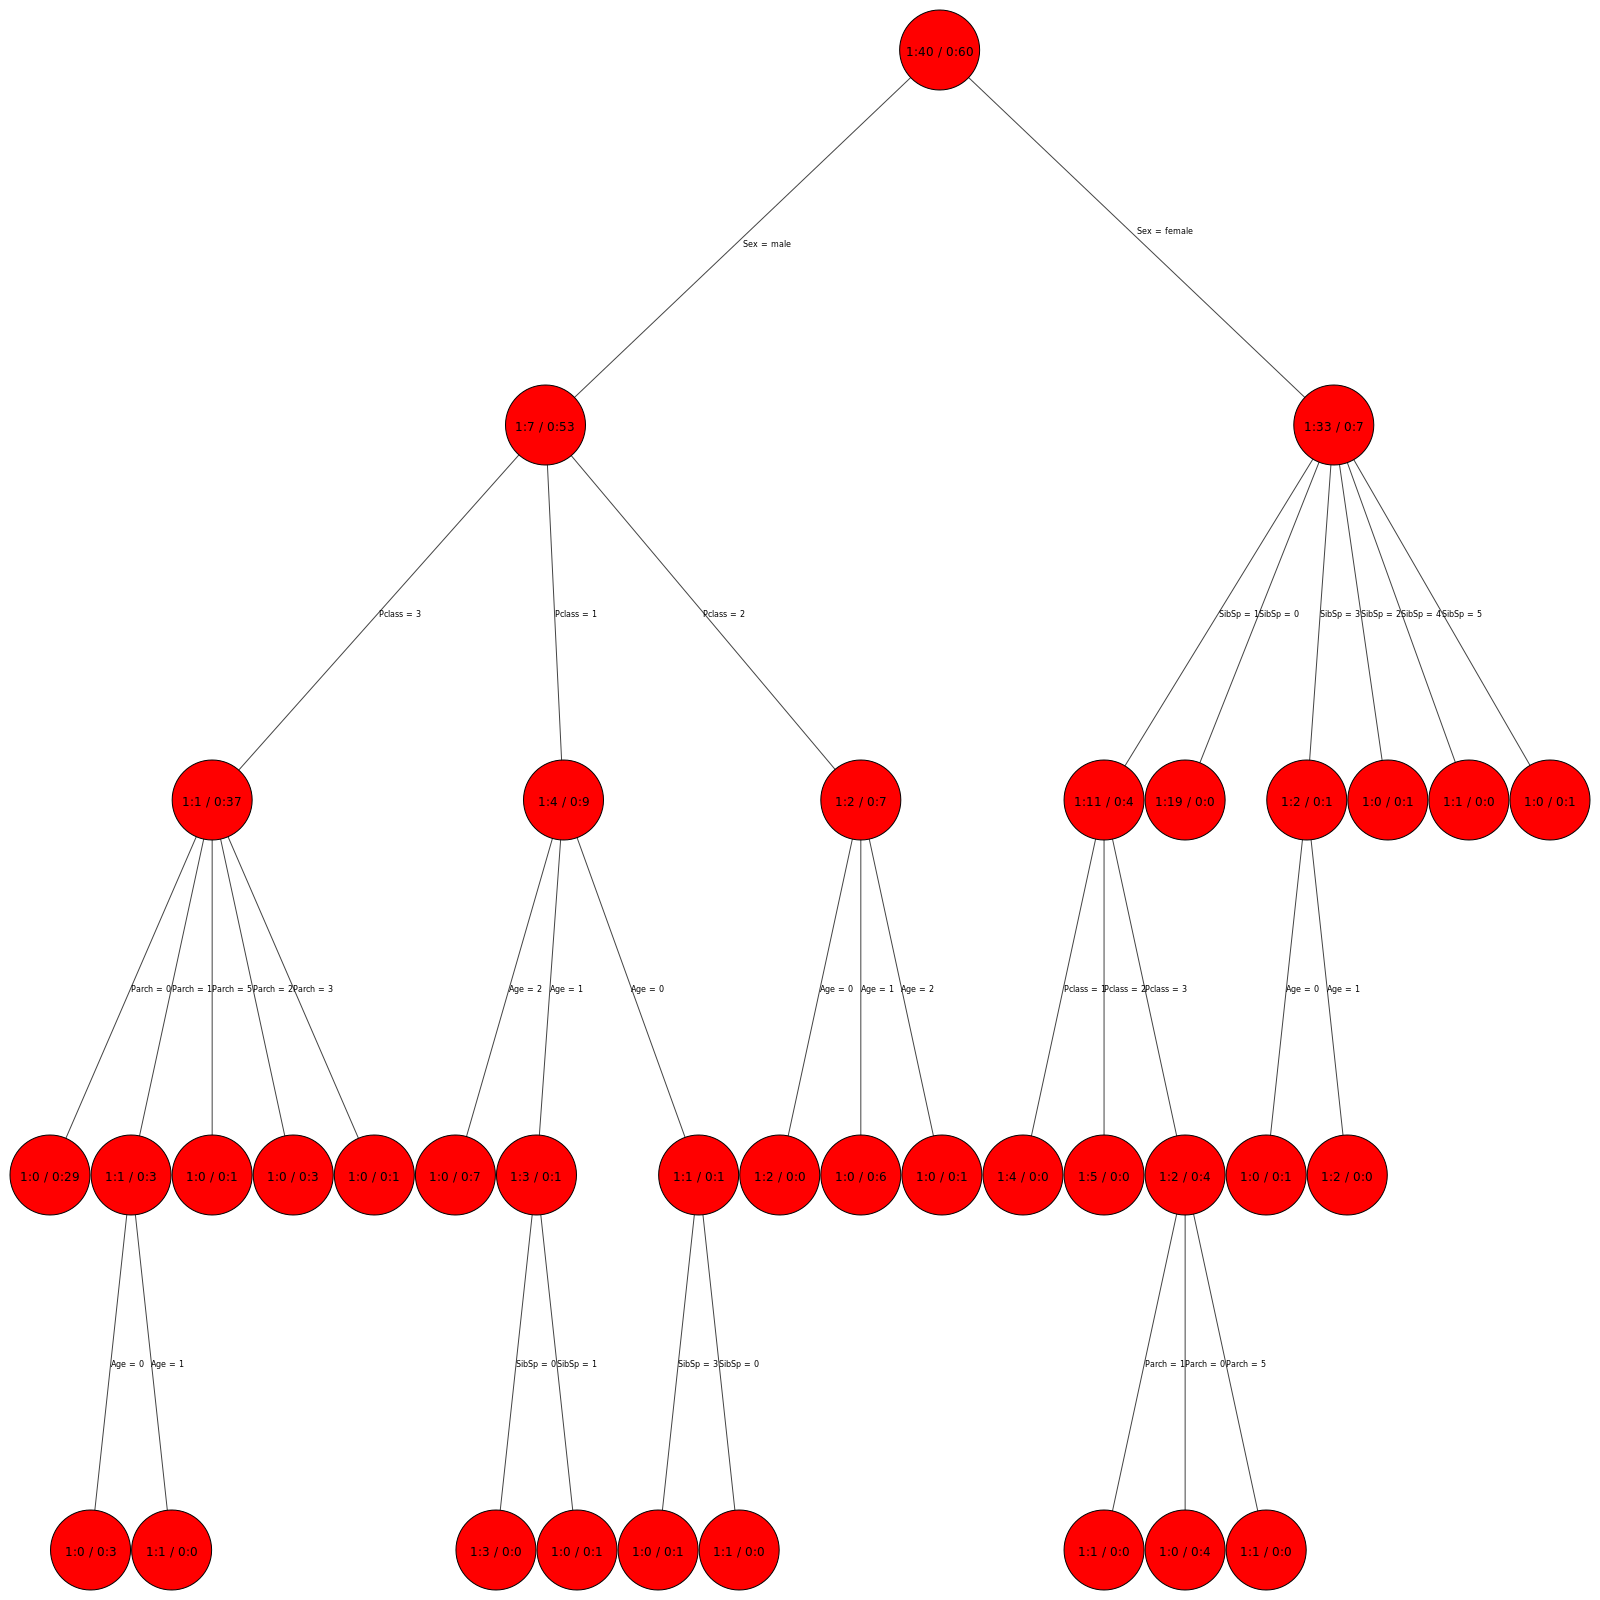
\includegraphics[width=\linewidth]{Dyskretny.png}
	\end{subfigure}
	\label{fig:dyskretne}
	\caption{Age jest atrybutem dyskretnym}
\end{figure}


\clearpage
\begin{figure}[h!]
	\subsection{Ciągły Age}
	\centering
	\begin{subfigure}[b]{1\linewidth}
		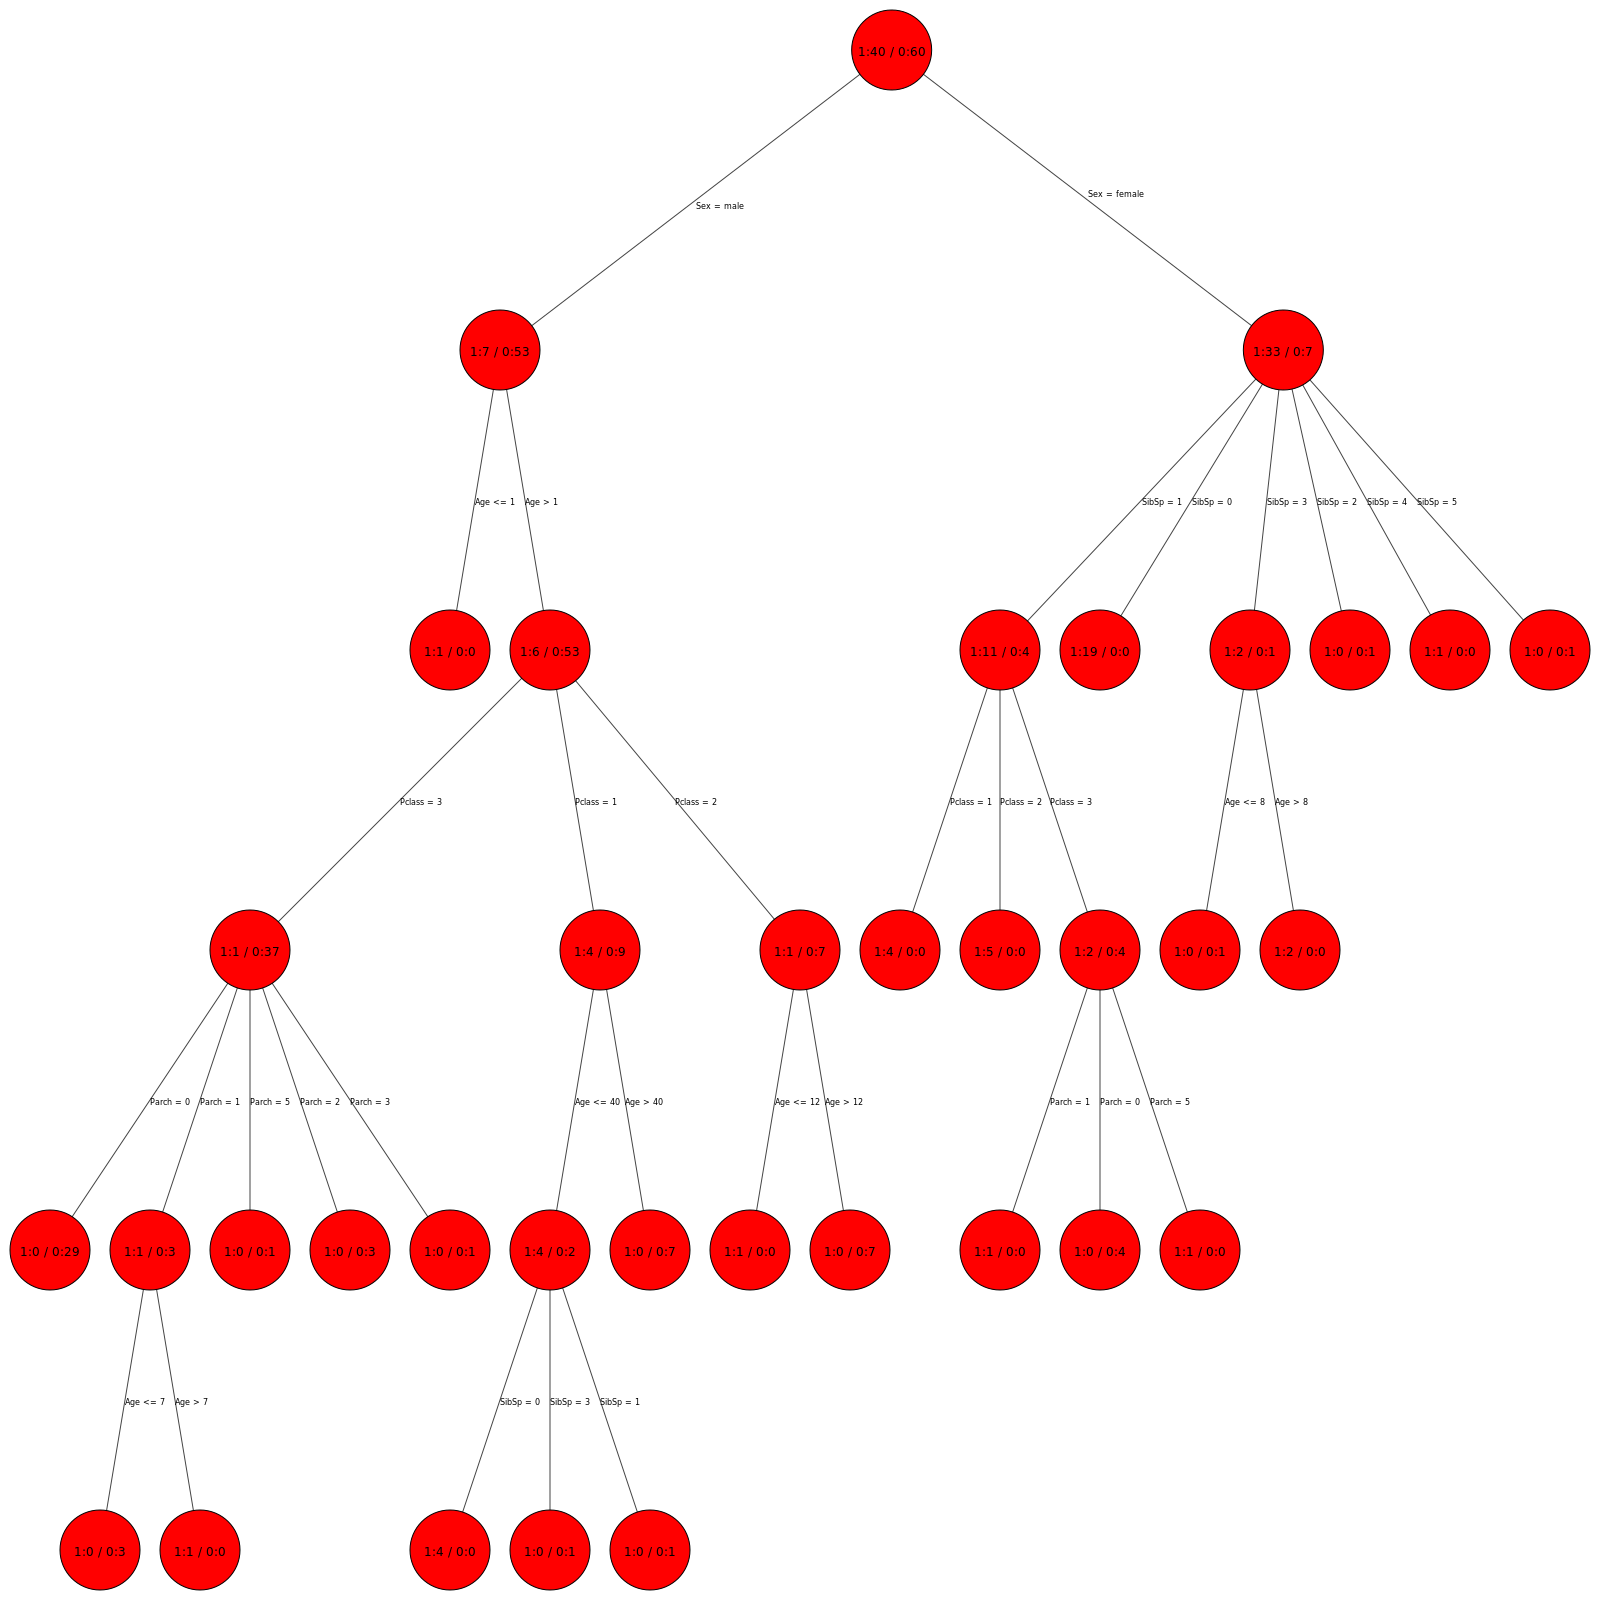
\includegraphics[width=\linewidth]{Ciagly.png}
	\end{subfigure}
	\label{fig:ciagle}
	\caption{Age jest atrybutem ciągłym}
\end{figure}

\end{document}
